% !TeX root = 场论与凝聚态.tex
There might be a puzzle through the derivation above, 
\begin{quote}
    \emph{Before integrating out $\pi$, the $\exp$ term contains $\pi \mathrm{i} \partial_{\tau} \phi$. This match seems presentation-depending.
    How to figure out this mapping in a presentation independent way?}
\end{quote}


\subsection{General Development}
We' ve seen that a quantum field theory in $d+1$-dim spacetime can be reinterpreted as a $d$-dim space statistic field theory by regarding the time dimension as a inverse temperature, but it is not so obvious when we did not mop up the integration of conjugate momenta $\pi$. We need to find a way in whole, to figure out in what situation a quantum field theory can be seen as a statistic field theory. \emph{``Just as the time when we heard about the formalism of Lagrangian mechanic, all cumbersome processes of force analysis disappeared.''}

\textbf{The answer is by locality and unitarity.}

Let us first compare the behaviors between QFT and stat. mech.
\footnote{
    The properties mentioned in the table are only valid with an implicit assumption that the base manifold of the field is orientable.
}
\begin{center}
    \begin{tabular}{|c|c|}
        \hline
        Real time & Imaginary time\\ 
        \hline & \\
        unitarity & reflection positivity\\ & \\
        \hline & \\
        \parbox{5cm}{\centering
            $\left( \mathrm{e}^{- \mathrm{i} H \Delta t} \right)^{*} = \mathrm{e}^{ - \mathrm{i} H (- \Delta t) }$
            \\
            $\Downarrow$
            \\
            $\mathop{\mathcal{Z}_{\mathbb{R} \times \Sigma}^{*} = \mathcal{Z}_{\mathop{\bar{\mathbb{R}}}\limits^{}_{\uparrow} \times \Sigma}}\limits^{}_{
                \hspace{5em} \text{orientation inversed}
                }
            $
            }&
        
        \parbox{5cm}{\centering
            also true because the only imaginary part is $\mathrm{e}^{- \int \mathrm{d} \tau \, \pi \mathrm{i}  \partial\tau \phi}$
            \\
            $\implies \mathcal{Z}^{*}_{\Sigma'} = \mathcal{Z}_{\bar{\Sigma}'}$
        } \\ & 

        \\ \hline

        \multicolumn{2}{|c|}{}\\

        \multicolumn{2}{|c|}{
            \parbox[h]{15cm}{The partition function of a locally defined theory can be splited into two parts, each on half of the base manifold. 
            For $\Sigma = \parbox{2.8cm}{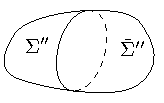
\includegraphics{figures/orientable_base.pdf}}$,
            the degree of freedom is the arbitrary boundary condition on $\partial \Sigma''$.
            By treating $\mathcal{Z}_{\Sigma''}$ and $\mathcal{Z}_{\bar{\Sigma}''}$ as functionals of $\left. \phi \right|_{\partial \Sigma''}$.
            we have 
            $$
            \mathcal{Z}_{\Sigma'} = \int  \left.\mathcal{D} \phi \right|_{\partial \Sigma''} \mathcal{Z}_{\Sigma''} \mathcal{Z}_{\bar{\Sigma}''} = \int  \left.\mathcal{D} \phi \right|_{\partial \Sigma''} \left( \mathcal{Z}_{\Sigma''} \right)  ^{2} \ge  0
            $$
            } 
        }\\
        \multicolumn{2}{|c|}{}\\
        \hline & \\

        \parbox{6cm}{\centering
            time reversal invariant \\
            $\Downarrow$ \\
            $\begin{cases} 
                \mathcal{Z}_{\Sigma' \times \bar{\mathbb{R}}} = \mathcal{Z}_{\Sigma' \times \mathbb{R}} \\
                \mathcal{Z}_{\Sigma'}^{*} = \mathcal{Z}_{\bar{\Sigma}'}
              \end{cases}
            $\\
            $\Downarrow$ \\
            $\mathcal{Z}$ is always real.
            }&
        \parbox{6cm}{
            \centering also \\ (useful in \emph{topological insulator})
            }
            \\ & \\
            \hline
        
    \end{tabular}
\end{center}
\clearpage
We have came to the conclusion that a theory with locality (of course with Hermitian Hamiltonian whilst) is always accompanied by a real and positive partition function $\mathcal{Z}$.



In the following it will be convinced that \emph{if and only if} the generative functional of a Euclidean field theory is real and positive, it has a \emph{classical stat. mech. interpretation}.

Sufficiency can be easily verified, as we have
\begin{equation}
  \mathcal{Z} = \int \mathcal{D} \phi  \, \exp\left( - \beta \int \mathrm{d} ^{d+1} r' \, \mathcal{H}(\phi) \right),
\end{equation}
no imaginary part appears in the expression of $\mathcal{Z}$.
\footnote{The integration of $\mathcal{D} \phi $ can be approximated by summation on a large amount of field configurations, which turns out to be Mont Carlo method for stat. mech.}

Proof of necessity is carried out by utilizing locality, as path integral can be performed in a certain subset on spacetime.\footnote{but there's no locality in momentum space.}
\begin{figure}
    \centering
    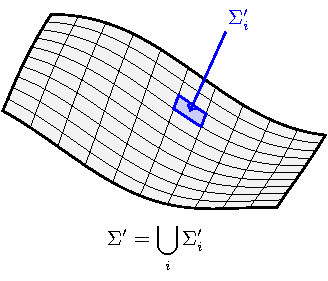
\includegraphics{figures/splited_base_manifold.pdf}
    \caption{Splited base manifold}
    \label{split_manifold}
\end{figure}
Splitting the base manifold into small parts, as shown in Fig\ref{split_manifold}, the path integral on each sub-manifold is fully determined by the b.c. on each $\partial\Sigma'_{i}$. Hence the path integral on $\Sigma'$ can be expressed as
\begin{equation}
    \mathcal{Z}_{\Sigma'} = \int \left( \text{b.c. of all boundary} \right) \prod_{i} \mathcal{Z}_{\Sigma' _{i} \text{ (b.c.)}}.
\end{equation}
Given that locality and unitarity guarantee that all $\mathcal{Z}_{\Sigma'_{i}}$ are \emph{real and positive}, such $\mathcal{Z}_{\Sigma'_{i}}$ is undoubtedly doable to be turned into the form of $\mathrm{e}^{- \tilde{\beta} \left( \cdots \right) }$, thus there always exists an effective Hamiltonian density and corresponding inverse temperature to match this QFT with a stat.~mech. interpretation.


\section[When do Symmetries Break Spontaneously]{SSB: What is Broken? Why no Tunneling?}

A name of ambiguity was designated to refer as the physical picture behind SSB, resulting a widespread misconstruction among juvenile learners, that ``\emph{a potential with minimal value at non-zero field strength will lead to SSB as vacuum state is static and tends to minimize its Hamiltonian, so it has to pick a state.}'' But such explanation will be no longer compatible if one try to replicate this in a statistic field theory and he would eventually figure out that $\left< s \right> = 0$. What on earth is broken!

To answer the question of what is breaking, we need to investigate a simplest case, that is, a $0$-dim field. 
\begin{figure}[hp]
    \centering
    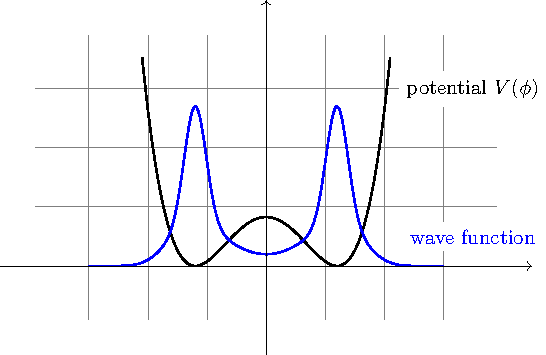
\includegraphics{figures/double_minimum_potential.pdf}
    \caption{$1$-dim field in a double-minimal potential}
    \label{1d_double_minimal}
\end{figure}
The picture of a $0$-dim field is generally characterized by Fig\ref{1d_double_minimal}. Directly from the figure, one can discover that the vacuum expectation value of $\phi$ is $0$, even though the field is trapped in a potential with two valleys. The key is that as long as the shape of potential is not so sharp, a non-zero tunneling amplitude will gradually expunge any symmetry-broken state as time evolutes. We need to get a approach to form a \emph{naturally} infinite potential barrier, i.e. at least one parameter of the system should be literally infinite.

In a system with infinite degrees of freedom, we describe it by a Hamiltonian density, thus
\begin{equation}
    V\left( \phi=0 \right) \propto \text{ volume of space}.
\end{equation}
Hence, a spontaneous symmetry broken only appears under \emph{thermodynamic limit}, and the dimension of base manifold should be greater than $2$ in stat. mech., which would be discussed later.

In the following we need to develop a well-defined language of SSB, since the ambiguity of describing SSB as a shifted vacuum expectation field strength will keep bothering us as long as we are about to investigate phenomena of SSB in stat. mech.

Taking ferromagnet as an example, a double-minimum potential would lead to degeneracy of ground state. To avoid vagueness in physical picture, we introduce a background magnetic field $B$, and consider the behavior of magnet strength in such case. 
There will be a susceptibility divergence in presence of SSB, equivalently infinitesimal change of $B$ leads to a finite change of $M$.(Fig \ref{magnetization of two phases})
\begin{figure}
    \centering
    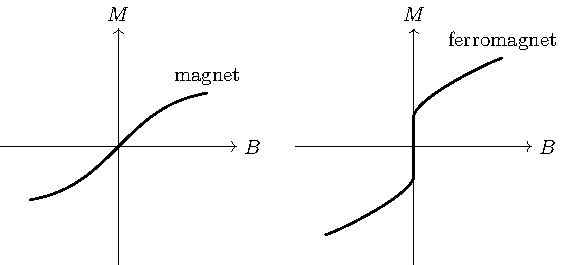
\includegraphics{figures/phase_transition_of_ferromagnet.pdf}
    \caption{Magnetization curve of two phases}
    \label{magnetization of two phases}
\end{figure}

By definition, we have
\begin{equation}
  M = \frac{\partial F}{\partial B}
\end{equation}
thus, a discontinuity of $M$ is corresponded to a non smoothness of shape $F$.

